\chapter{Statement Coverage}

\section{Introduction}

This chapter details my effort to implement statement coverage for EOL programs. I begin by analysing the Epsilon source code that I will be working with. I then move on to detailing the design and implementation of the solution. Then I move onto testing the solution, and finish off with a conclusion on the successes and failures of the solution.

\section{Analysis}

The Epsilon source is broken into many well-organised packages. The packages \verb+org.eclipse.epsilon.eol.*+ contain all of the code that is specific to the EOL language, and so these will be the primary focus of this analysis.

The package \verb+org.eclipse.epsilon.eol.execute+ unsurprisingly contains the code to execute an EOL program. To perform statement coverage, it is necessary to determine which statements have been executed. 

Some analysis of the execute package and its sub-packages has uncovered the interface \verb+IExecutionListener+, as shown in Figure \ref{lst:IExecutionListener}. An instance of a class that implements this interface can be added to a list of execution listeners. When a statement is about to execute, each object in the list has its \verb+aboutToExecute+ method called, and similarly after each statement has executed, each object in the list has its \verb+finishedExecuting+ method called.

\begin{figure}
	\lstinputlisting[language=java]{code/IExecutionListener.java}
	\caption{The public interface IExecutionListener}
	\label{lst:IExecutionListener}
\end{figure}

In the literature review the purpose of an Abstract Syntax Tree (AST) was described. The first parameter of both methods in \verb+IExecutionListener+ is an abstract syntax tree object. The Abstract Syntax Tree class in Epsilon is designed in such a way that each vertex is an object of type AST, and each vertex has a list of children vertices, as well as a pointer back to the parent vertex. The parent vertex will have a null pointer in place of a pointer to a parent vertex, and leaf of the tree will have an empty list of children.

The AST object that is passed as a parameter into both functions is a pointer to the vertex in the program's abstract syntax tree that is about to be executed or has just been executed, depending on the method being called. 

\begin{figure}
\centering
\begin{minipage}{.5\textwidth}
  \centering
  \lstinputlisting[language=EOL]{code/HelloWorld.eol}
  \caption{A simple EOL program}
  \label{lst:helloWorldEOL}
\end{minipage}%
\begin{minipage}{.5\textwidth}
  \centering
  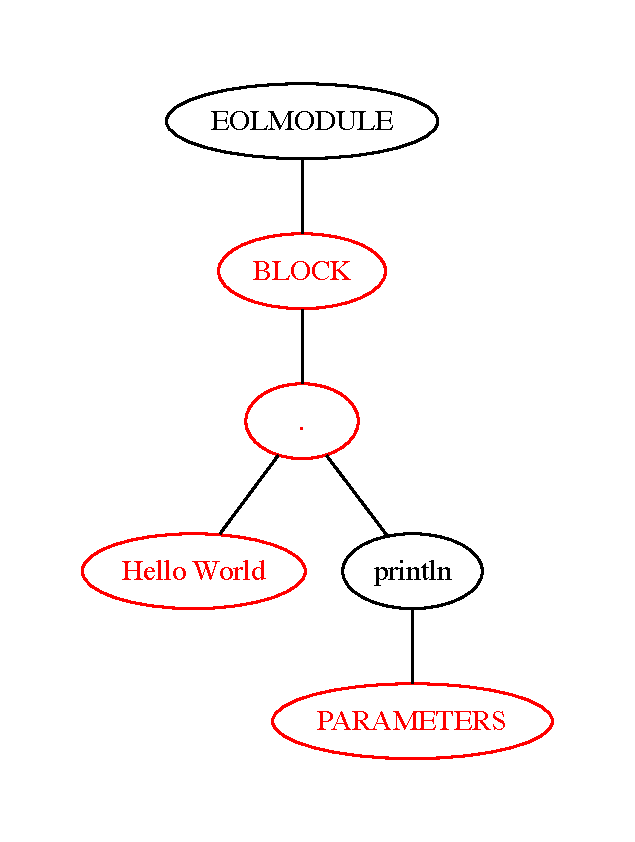
\includegraphics[scale=0.5]{figures/HelloWorldAST.pdf}
  \caption{The AST of the program in Figure \ref{lst:helloWorldEOL}}
  \label{fig:helloWorldAST}
\end{minipage}
\end{figure}

One approach for determining how many statements were executed would be to keep a list of visited AST vertices, and then count the total number of vertices in the AST. There is however a problem with this approach: Consider the very simple code in Figure \ref{lst:helloWorldEOL}, and the AST that is generated for the simple program as shown in Figure \ref{fig:helloWorldAST}. With that simple program, there is only 1 line that is going to be executed because there are no conditional statements that cause the program flow to change. However, the AST is comprised of 6 vertices. Testing shows that the execution listener's methods are only called on the red vertices. So while we know that the whole program has been executed, this naive approach will report only 4 out of 6 vertices have been executed.

Another approach that could be considered is to record which lines of the input file have been executed. This can be done because the AST class has a method called \verb+getLine()+ which as you would expect returns the line on which that statement comes from. So all of the red highlighted edges in Figure \ref{fig:helloWorldAST} return line 1 when \verb|getLine()| is called. So initial analysis would suggest that 1 out of 1 lines has been covered in the simple program in Figure \ref{lst:helloWorldEOL}, which is accurate. The problem with this was discussed in the literature review, and that is that it relies on two statements not being placed on the same line. The code in Figure \ref{lst:ifElseEOL} and its accompanying AST in Figure \ref{fig:ifElseAST} demonstrate this problem. Line coverage correctly is 100\%, because 1 out of 1 lines have been executed. However, not all of that 1 line has been executed, and so this is not an accurate reflection of the coverage. With the AST, 7 out of 14 vertices have been executed, which is a lot more accurate than the line coverage.

\begin{figure}
\centering
\begin{minipage}{.5\textwidth}
  \centering
  \lstinputlisting[language=EOL,breaklines=true]{code/ifElse.eol}
  \caption{An if/else EOL program}
  \label{lst:ifElseEOL}
\end{minipage}%
\begin{minipage}{.5\textwidth}
  \centering
  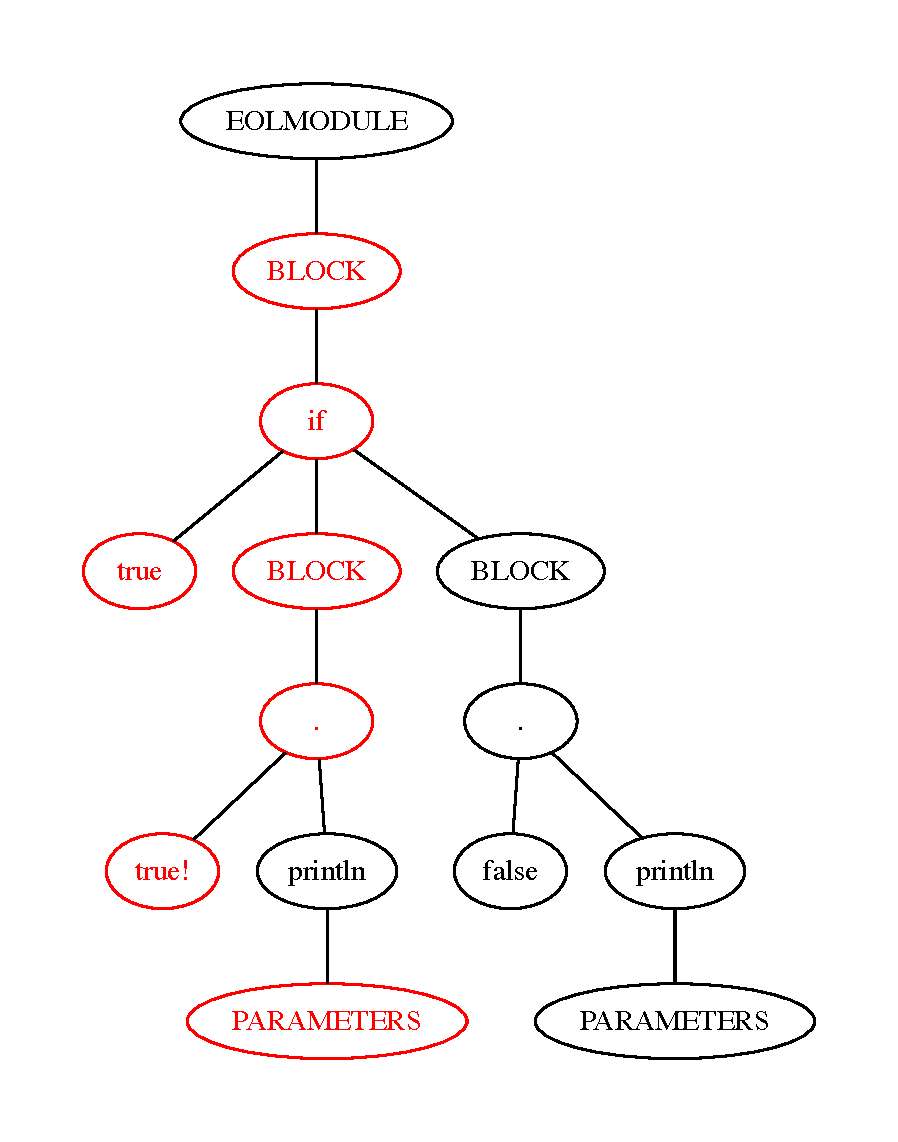
\includegraphics[scale=0.5]{figures/ifElseAST.pdf}
  \caption{The AST of the program in Figure \ref{lst:ifElseEOL}}
  \label{fig:ifElseAST}
\end{minipage}
\end{figure}

Thankfully another option is available. The AST class has a method called \verb|isImaginary()| which returns true when the current vertex is `imaginary'. While no documentation is available, it appears that vertices that can be directly mapped back to some text from the input file are not imaginary, and those that cannot be mapped back to some text are not. Figure \ref{fig:ifElseASTreal} shows the AST again, but this time with imaginary vertices left white, while non-imaginary vertices are filled in yellow. Quickly it becomes apparent that the definition of the method \verb+isImaginary()+ is not perfect as the vertex labelled EOLMODULE is coloured in yellow, despite not being directly mappable to a single statement in the input code. 

\begin{figure}
	\centering
	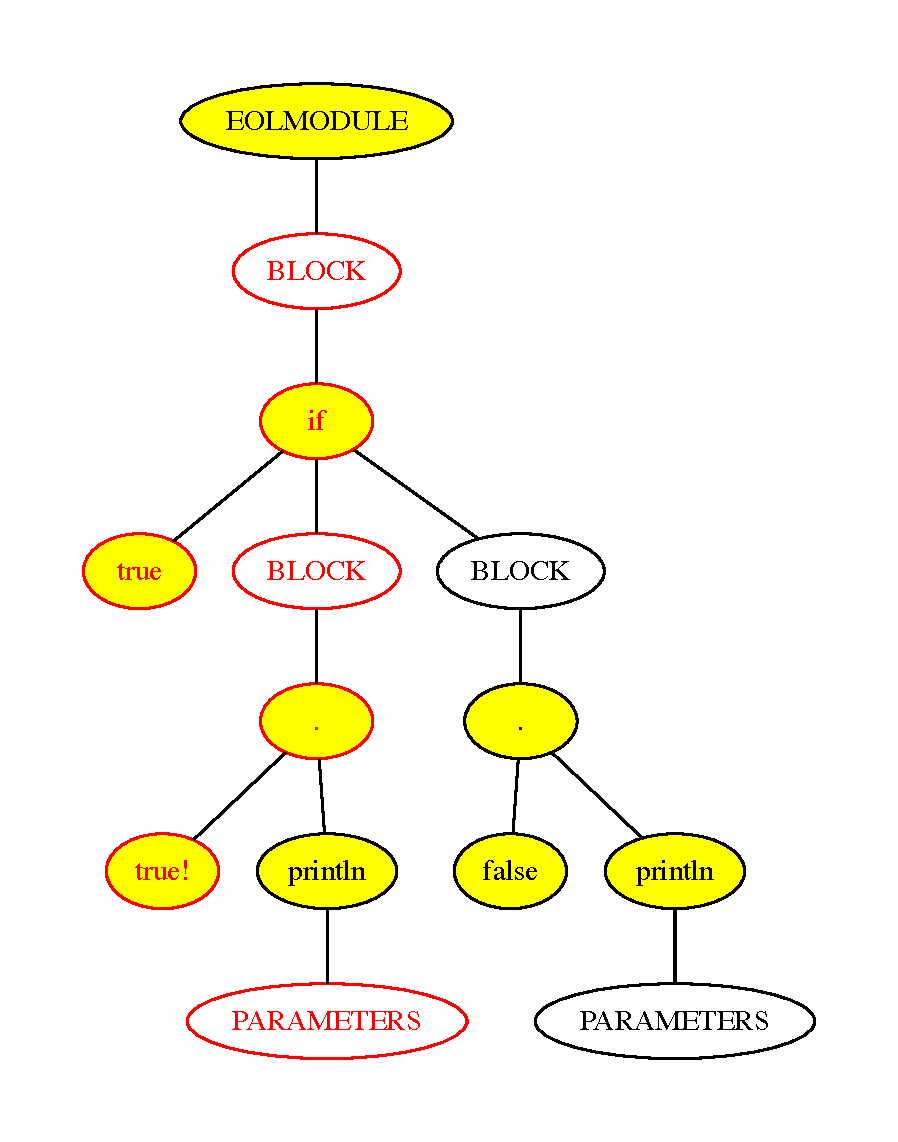
\includegraphics[scale=0.5]{figures/ifElseRealAST.pdf}
	\caption{The AST with yellow vertices being `real', and white vertices being `imaginary'}
	\label{fig:ifElseASTreal}
\end{figure}

\section{Design}

When the EOL executor calls the execution listener's pre or post execute methods, there needs to be a way to store a reference to the AST that is passed into either of the methods.

An obvious way of doing this would be to have a list of references to the AST. When one of the pre or post-execute methods is fired, a check would be performed on the list to see if a reference to that particular AST vertex was already stored, and if not, it would be added to the list.

Once the program has completed execution, in order to satisfy requirements F-03 and F-04, an analysis must then be performed to determine which vertices have been executed, and which have not. To do this, each vertex in the AST must be checked against the list of visited vertices. The AST can either be traversed by a depth or breadth-first algorithm. I have chosen to use a depth-first algorithm purely because it is easier to implement, and uses less storage space than the breadth-first (as no queue has to be stored).

At each recursion in the depth-first traversal, the list of visited vertices must be checked against the current vertex. This is therefore a O($n^2$) algorithm, which is not ideal as any sizeable programme can quickly slow down, which goes against requirement NF-01. 

A way around this problem then is to use a hashmap to store the visited vertices. When either the pre or post-execute methods of the execution listener are fired, the hashmap would use the AST instance as the key, and the value would be a boolean. To insert to the hashmap, the values \verb|<ast, true>| would be passed in (where \verb|ast| is the AST instance). Later during analysis, a simple call of the Java HashMap method \verb|containsKey| would suffice, as it would return true if the AST instance has been inserted into the hashmap, or false otherwise. The use of a boolean as the value is arbitrary and in fact any value would suffice. 

This approach better fits the requirement NF-02, although NF-01 could potentially still not be met. If the default hashing function is poor and causes many collisions then the performance could degrade to a similar level of the previously described approach using a list of references. A solution could be to implement a better hashing function, but it seems like a lot of effort for what may not even be a problem.

Both of the above solutions work around the Epsilon source code by storing information in new objects. However this is not actually a requirement - it is perfectly acceptable to modify the Epsilon code as long as it is justifiable. The most simple solution then is to modify the AST class so that it contains a boolean that stores whether or not that particular vertex has been executed. When initialised of course this boolean will be set to false, but when the post-execute function in the execution listener is called and it is passed an AST as a parameter, we can just change the value of the executed boolean within the AST. This has the advantage of meaning that recording that a vertex has been visited is guaranteed to be a O(1) operation (unlike the hashmap or list based solutions). Better still, when the analysis is performed after execution has completed, the lookup time to determine whether a vertex has been executed is also guaranteed to be O(1). Again this is unlike the hashmap or linked list based solutions, which were worst case O(n) lookup time.

With the core algorithms decided on, the structure of the actual code has yet to be decided upon, as well as the output from the code. There of course needs to be a class that implements the \verb|IExecutionListener| interface. As the AST is directly being modified, then there is no need to transfer any data out of the execution listener (the AST will be available through another module). There therefore needs to be a class that takes the AST as input, and produces output of some sort. So to summarise, there will be two classes implemented. One called \verb|StatementCoverageListener| that implements the execution listener interface, and another called \verb|StatementCoverageAnalyser| that analyses and outputs some information.

The format of the output must satisfy requirements F-03 and F-04, that is that it will tell the user how many statements were executed, and it will also tell the user which statements were executed, and which were not. For the latter, research detailed in the literature review of other coverage tools shows that a popular way to do this is by highlighting the statements that were executed, and either leaving statements unhighlighted that have not been executed, or highlighting them in a different colour. Most of these tools worked as plugins to the Eclipse user interface. However, this is a lot of work and time is limited, so initially I will find a quicker approach. If time permits, then I will create the plugin after all other work is finished.

An easy way to output formatted text is to use HTML. HTML is easy to generate programmatically, and rendering the text is outsourced to a web browser. It would be possible to build my own text viewer, but it seems overly complicated when there are no disadvantages to generating a HTML page.

I will create a class that takes as input the executed AST, the file that has been executed, and the file to write the HTML to. The class will have to map executed vertices to actual characters that are in the executed file. The AST provides a function that make this relatively simple - there is a \verb|getRegion| method that allows access to the start and end positions in the file of the statement that that AST vertex maps to. From this, we need to go through the input file and mark the statements that have been executed, and those that have not. There are two possible ways to go about this. 

The first approach is to go through the executed file character by character, and go through every node in the AST and find if that particular character maps to a vertex. If it does, and that vertex has been executed, then highlighting is enabled (by changing the text background colour in HTML), and the character is copied to the output file. If the character cannot be mapped to a vertex, or it can be mapped but the vertex was not executed, then the character is simply copied across to the output file. The disadvantage of this approach is that it will be very time consuming to traverse the whole AST for every single character in the executed file. This will not help to meet requirement NF-01.

A better approach then will be to store for every character in the input text file whether or not that character should be highlighted. Initially every character will be set to not highlighted, but then the AST will be traversed, and any nodes that are not imaginary and that have been executed, the character will be set to be highlighted. Once the traversal has completed, the executed file's contents will be copied character for character. If the character being copied has been marked as highlighted, then the HTML highlighting tag will surround the character. The disadvantage of this approach is that it will require more memory than the previous approach, as it is now necessary to store more information for each character. However, it will be significantly quicker than the other approach, as the AST will only need to be traversed once.

In order to satisfy F-02, there will be a main method in the output class that takes an EOL file and output file as input, and executes the EOL file and outputs HTML to the output file.

\section{Implementation}

The first step was to modify the AST class. The additions are shown in Figure \ref{lst:ASTStatementAdditions}. Two methods (a getter and setter) have been added to modify the new boolean variable.

\begin{figure}[h]
	\lstinputlisting[language=java]{code/AST_statement.java}
	\caption{Additions to the AST class}
	\label{lst:ASTStatementAdditions}
\end{figure}

Following that, a class that implements the execution listener interface was created, and the post-execute method was completed to set the AST node to being visited.

\begin{figure}[h]
	\lstinputlisting[language=java]{code/StatementCoverageListener.java}
	\caption{The StatementCoverageClass code}
	\label{lst:StatementCoverageListener}
\end{figure}

Finally, the HTML outputter class was implemented. The whole class is too large to include here, so certain interesting parts are documented. The whole class can be found in the source that is included with this project, in the folder ?

% TODO add folder!

\begin{figure}[h]
	\lstinputlisting[language=java]{code/statement_HTML_core.java}
	\caption{The core of the Statement Coverage HTML output class}
	\label{lst:StatementCoverageHTMLCore}
\end{figure}

The core of the class is detailed in Figure \ref{lst:StatementCoverageHTMLCore}. Going through line-by-line, it initially reads in every line of the input file into a list of Strings. Then it next fills in the `covered array', which is an array of strings that is exactly the same in size as the list of strings that holds the input file. So for each character in the input file, there is a position in the covered array that stores whether or not the character should be highlighted. Initially all positions in the covered array are set to a 'N' character. The function \verb|dfAST| then performs a depth-first traversal of the AST of the executed program. It counts the number of non-imaginary vertices, as well as counts the number of non-imaginary executed vertices. As well it also changes the appropriate characters in the covered array to a 'Y' when an executed statement is found. 

At this stage the AST has been traversed, and it is known which characters are to be highlighted and which are not to be. Now the HTML file is written. This is started by writing the HTML header, then the page title. Then the coverage statistics are written so to satisfy requirement F-03. Next, the code from the input file is copied to the output file, and the code that has been executed is highlighted. Finally, the HTML page footers are written and the file is written to disk.

\section{Testing}
Following the implementation of the solution, it must now be thoroughly tested for bugs, and of course if any bugs are found, then the fixes will be documented here.

\begin{samepage}
\begin{description}[style=sameline,leftmargin=3.5cm,nolistsep]
\item[\hspace*{0.3cm}Label] ST-01
\item[\hspace*{0.3cm}Description] A simple program that outputs `Hello, World'.
\item[\hspace*{0.3cm}Expected Output] 100\% coverage, all code highlighted.
\item[\hspace*{0.3cm}Result] Fail
\end{description}
\end{samepage}

Unfortunately the first test has failed. The output is shown in Figure \ref{fig:ST01HTML} shows this. For the test to pass, the coverage percentage should have been 100\%, but it is showing 66\%. All of the code is highlighted, which is correct. Analysis of the AST for the sample program is shown in Figure \ref{fig:ST01AST}. As before, yellow vertices are non-imaginary vertices that can be mapped to some text of the executed file, and vertices that are outlined in red are the ones that have been marked as executed. There is code in the analyser to ignore the \verb|EOLMODULE| vertex, which is why it is only counting 3 vertices. However, rather than the \verb|println| vertex being marked as executed, its child \verb|PARAMETERS| vertex has been marked as executed. This can also be seen to be the case in Figure \ref{fig:ifElseAST}, but was not spotted at the time. 

At this stage there are a few solutions available. The first is that some code can be added to check with a \verb|println| vertex whether or not its child \verb|PARAMETERS| vertex has been executed. While a quick solution, further investigation shows that other operations also suffer from the same issue. Another potential solution is to modify the code of Epsilon so that the execution listener's post-execute method is fired on the \verb|println| vertex rather than the \verb|PARAMETERS| vertex. Unlike the simple modification that was made to the AST class earlier, this is likely to be a big job, and is probably not ideal considering that easier solutions are available. I feel then that the best solution is to modify the execution listener to detect when it has been sent a \verb|PARAMETERS| vertex to actually mark the parent vertex as executed.

\begin{figure}
\centering
\begin{minipage}{.5\textwidth}
  \centering
  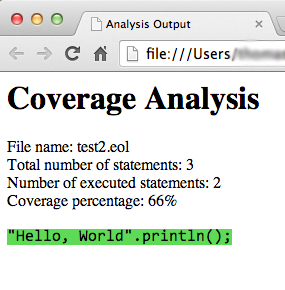
\includegraphics[width=0.6\linewidth]{figures/ST01HTML.png}
  \caption{The HTML output from test ST-01, shown in Google Chrome}
  \label{fig:ST01HTML}
\end{minipage}%
\begin{minipage}{.5\textwidth}
  \centering
  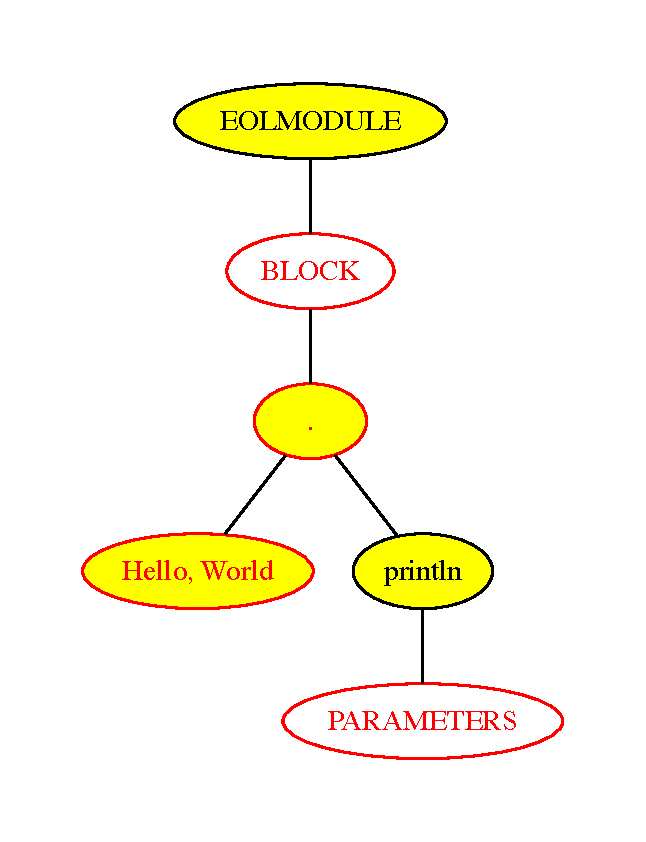
\includegraphics[width=0.6\linewidth]{figures/ST01AST.pdf}
  \caption{The AST for the program run in test ST-01}
  \label{fig:ST01AST}
\end{minipage}
\end{figure}

The code that was previously listed in Figure \ref{lst:StatementCoverageListener} has now been modified with the code shown in Figure \ref{lst:StatementCoverageST01Mod}.

\begin{figure}[h]
	\lstinputlisting[language=java]{code/statement_ST01_mod.java}
	\caption{The updated post-execution method}
	\label{lst:StatementCoverageST01Mod}
\end{figure}

The results from re-running test ST-01 are shown in Figure \ref{fig:ST01HTMLfixed}, and the AST is shown in Figure \ref{fig:ST01ASTfixed}. The test now passes.

\begin{figure}
\centering
\begin{minipage}{.5\textwidth}
  \centering
  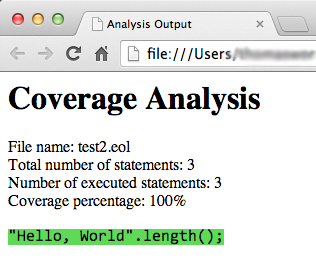
\includegraphics[width=0.6\linewidth]{figures/ST01HTML_fixed.png}
  \caption{The output after re-running test ST-01}
  \label{fig:ST01HTMLfixed}
\end{minipage}%
\begin{minipage}{.5\textwidth}
  \centering
  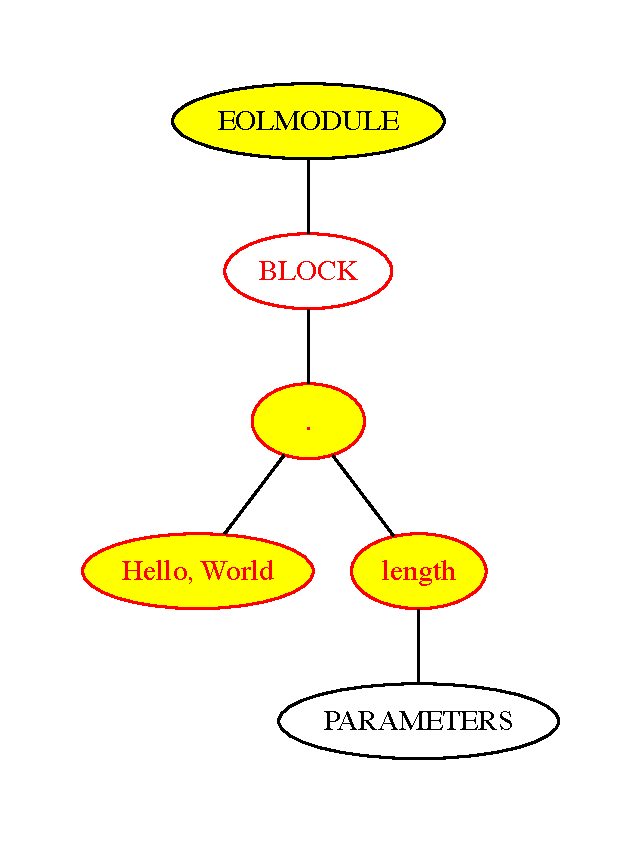
\includegraphics[width=0.6\linewidth]{figures/ST01AST_fixed.pdf}
  \caption{The AST for the program run in test ST-01}
  \label{fig:ST01ASTfixed}
\end{minipage}
\end{figure}

\begin{samepage}
\begin{description}[style=sameline,leftmargin=3.5cm,nolistsep]
\item[\hspace*{0.3cm}Label] ST-02
\item[\hspace*{0.3cm}Description] A single if-else statement, where the IF evaluates to true and so the contents of else never execute.
\item[\hspace*{0.3cm}Expected Output] Only statements within the IF block are executed, and only those statements are highlighted.
\item[\hspace*{0.3cm}Result] Pass
\end{description}
\end{samepage}

\begin{samepage}
\begin{description}[style=sameline,leftmargin=3.5cm,nolistsep]
\item[\hspace*{0.3cm}Label] ST-03
\item[\hspace*{0.3cm}Description] A single if-else statement, where the IF evaluates to false and so the contents of it never execute, but the contents of the else block do.
\item[\hspace*{0.3cm}Expected Output] Only statements within the ELSE block are executed, as well as the if evaluation.
\item[\hspace*{0.3cm}Result] Pass
\end{description}
\end{samepage}

\begin{samepage}
\begin{description}[style=sameline,leftmargin=3.5cm,nolistsep]
\item[\hspace*{0.3cm}Label] ST-04
\item[\hspace*{0.3cm}Description] A for-loop that contains a few statements, including one conditional statement that should execute on at least one iteration of the for-loop
\item[\hspace*{0.3cm}Expected Output] All statements within the for-loop should be highlighted.
\item[\hspace*{0.3cm}Result] Pass
\end{description}
\end{samepage}

\begin{samepage}
\begin{description}[style=sameline,leftmargin=3.5cm,nolistsep]
\item[\hspace*{0.3cm}Label] ST-05
\item[\hspace*{0.3cm}Description] Both a context-free and context operation are defined and called.
\item[\hspace*{0.3cm}Expected Output] All statements within each operation should be executed.
\item[\hspace*{0.3cm}Result] Pass
\end{description}
\end{samepage}

\section{Conclusions}

While the tests are highlighting the code correctly, it is notable that the covered percentage value is not actually of much use to a developer. Some statements are never actually executed, and so coverage is rarely 100\%. For ST-01 this was the case and was fixed, but further testing has shown that the problem is quite widespread. The output for ST-05 is shown in Figure \ref{fig:ST05HTML}, and the corresponding AST in \ref{fig:ST05AST}. The AST is significantly larger than in previous examples, but upon close inspection there are vertices that are classed as non-imaginary, that are not executed, despite the program being fully executed. Having considered this problem, I have concluded that the output is technically accurate, and thus meets requirement F-03. 

Furthermore, F-04 is satisfied as it is easy to distinguish which code has been executed and what has not. With test ST-05 the user will want to see that the contents of both operations have been executed, as well as the first line that calls the operations. The fact that the operation headers are not fully covered is unlikely to be of use to the developer, and so I do not believe that this is an issue.

Requirement F-02 has been satisfied, as the main method in the HTML output class takes in an EOL file and executes it. 

Anecdotal evidence suggests that NF-01 and NF-02 have also been satisfied. Further analysis of this may be required at a later date however.

\begin{figure}
\centering
\begin{minipage}{.5\textwidth}
  \centering
  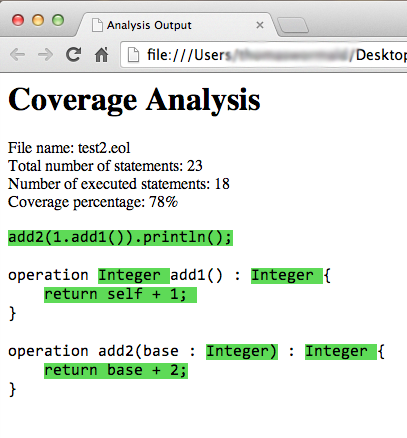
\includegraphics[width=0.6\linewidth]{figures/ST05HTML.png}
  \caption{The output after from test ST-05}
  \label{fig:ST05HTML}
\end{minipage}%
\begin{minipage}{.5\textwidth}
  \centering
  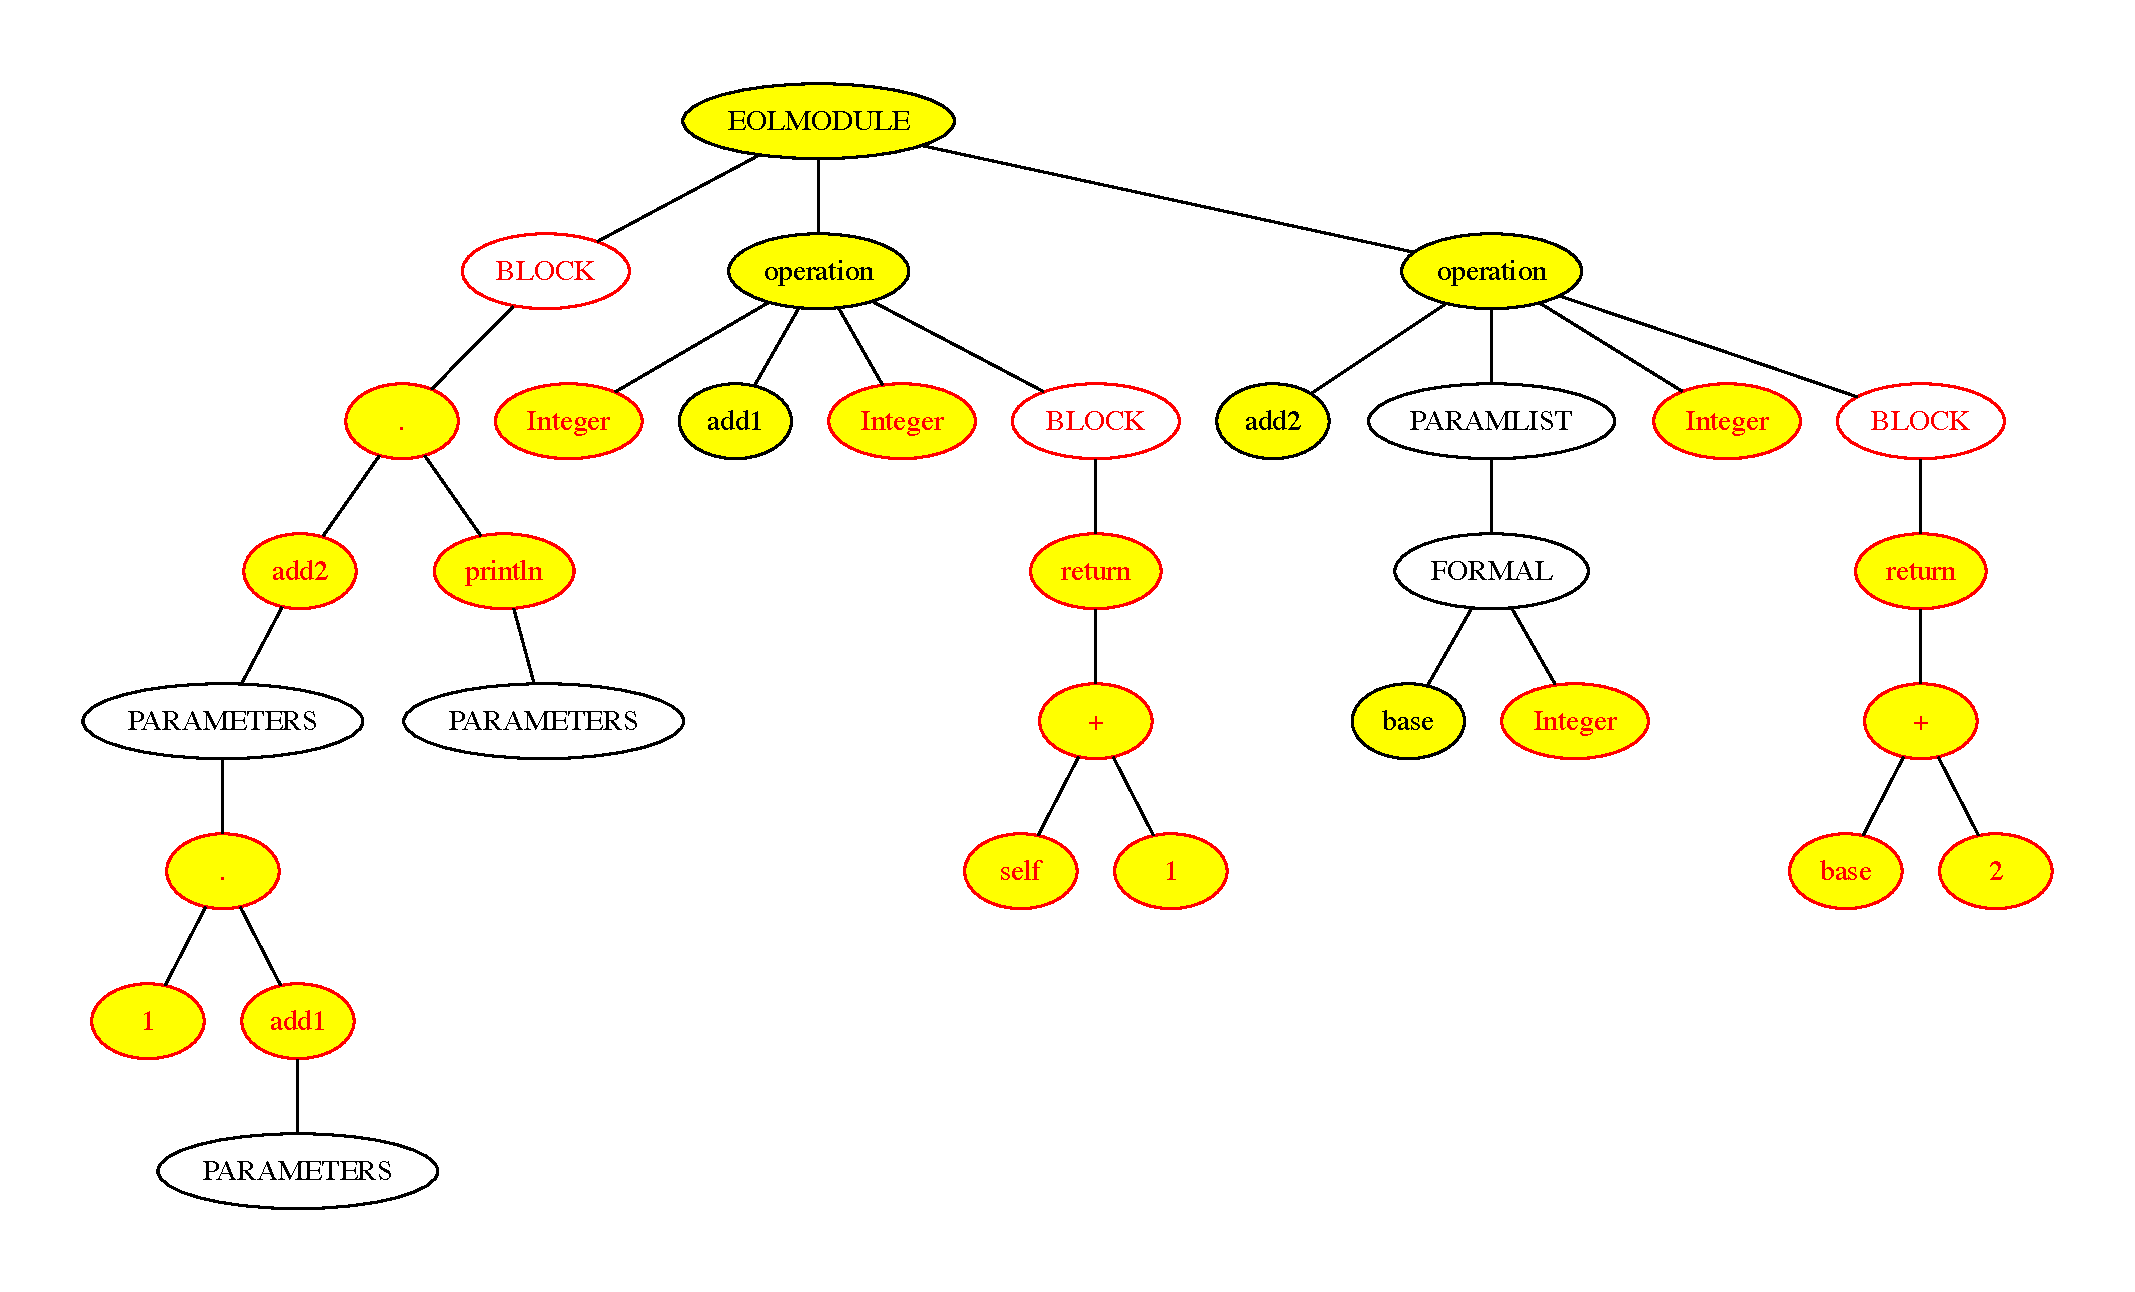
\includegraphics[width=\linewidth]{figures/ST05AST.pdf}
  \caption{The AST for the program run in test ST-05}
  \label{fig:ST05AST}
\end{minipage}
\end{figure}
